\section*{Figure Legends and Figures}

\begin{figure}[!ht]
\centering
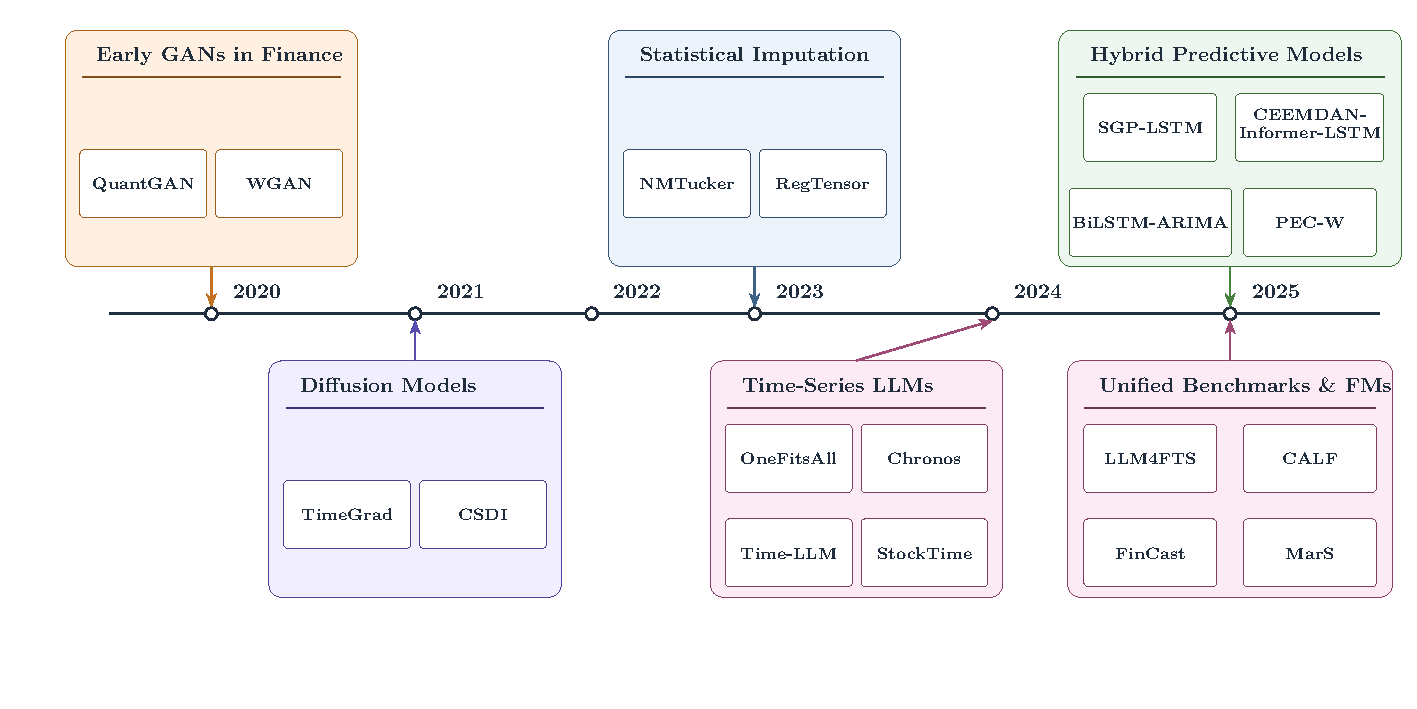
\includegraphics[width=0.98\linewidth]{separate_figures/Figure1.pdf}
\caption{\textbf{Evolution of Financial Time-Series Generation techniques over the past decade.} Timeline of representative milestones in financial time-series generation (FTSG) from 2020 to early 2026. Colored cards along the central axis denote technical families: coral pink for adversarial generative architectures (GANs), steel blue for diffusion and score-based models, amber orange for time-series foundation models and adapted large language models (LLMs), and sage green for classical statistical, tensor factorization, and deep predictive baselines. Key models include NMTucker (Non-negative Matrix Tucker factorization), RegTensor, NDDP (Nonlinear Diffusion Drift Process), PEC-W, SGP-LSTM, TimeGrad, CSDI, Time-LLM, StockTime, CALF (Cross-modal Aligned Foundation model), FinCast, and MarS (Multi-Agent Market Simulator). White circular markers denote calendar years 2020, 2021, 2023, 2024, and 2025; directed arrows align each contribution to its release year.}
\label{fig:timeline}
\end{figure}

\newpage

\begin{figure}[!ht]
\centering
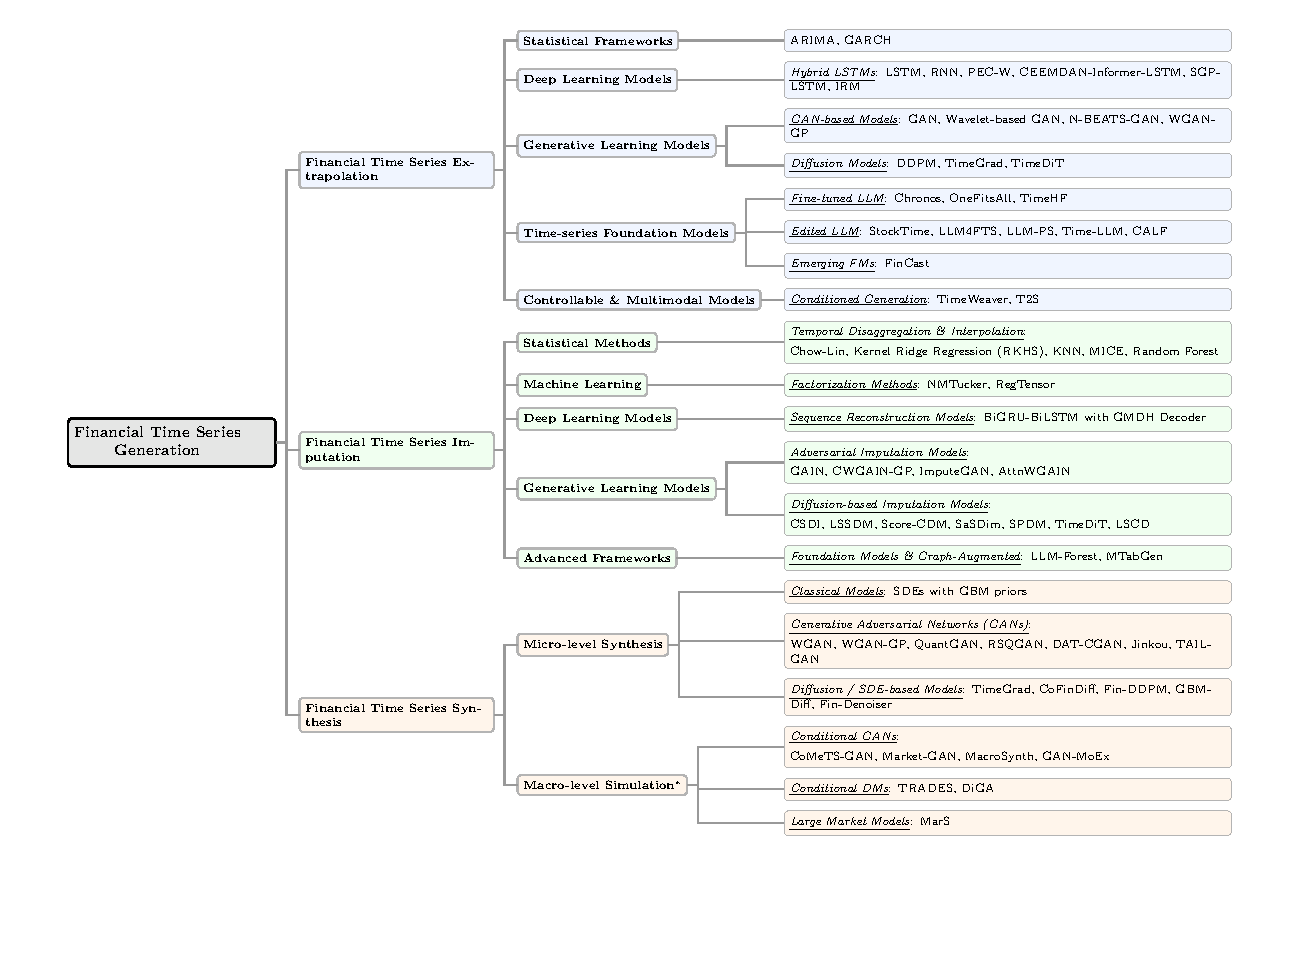
\includegraphics[width=0.98\linewidth]{separate_figures/Figure2.pdf}
\caption{\textbf{Hierarchical two-level taxonomy of financial time-series generation.} Systematic classification structure decoupling financial generation tasks from generative modeling paradigms. The primary tree root partitions FTSG into three functional task branches. Light blue shaded blocks designate the forward-looking Financial Time-Series Extrapolation (FTSE) branch, spanning statistical autoregressive models, deep sequential networks, adversarial frameworks, diffusion dynamics, and foundation model adaptations. Light green shaded blocks designate the bidirectional Financial Time-Series Imputation (FTSI) branch, covering temporal disaggregation, tensor factorization baselines, recurrent encoders, generative adversarial imputers, score-based diffusion methods, and graph-augmented transformer architectures. Light orange shaded blocks designate the generative Financial Time-Series Synthesis (FTSS) branch, categorized into micro-level asset return synthesis and macro-level market microstructure simulation across conditional GANs, diffusion models, and large market agent simulators. Grey orthogonal branch lines indicate conceptual inheritance. The asterisk ($^*$) indicates that only purely generative model families are enumerated in the synthesis branch.}
\label{fig:taxonomy}
\end{figure}

\newpage

\begin{figure}[!ht]
\centering
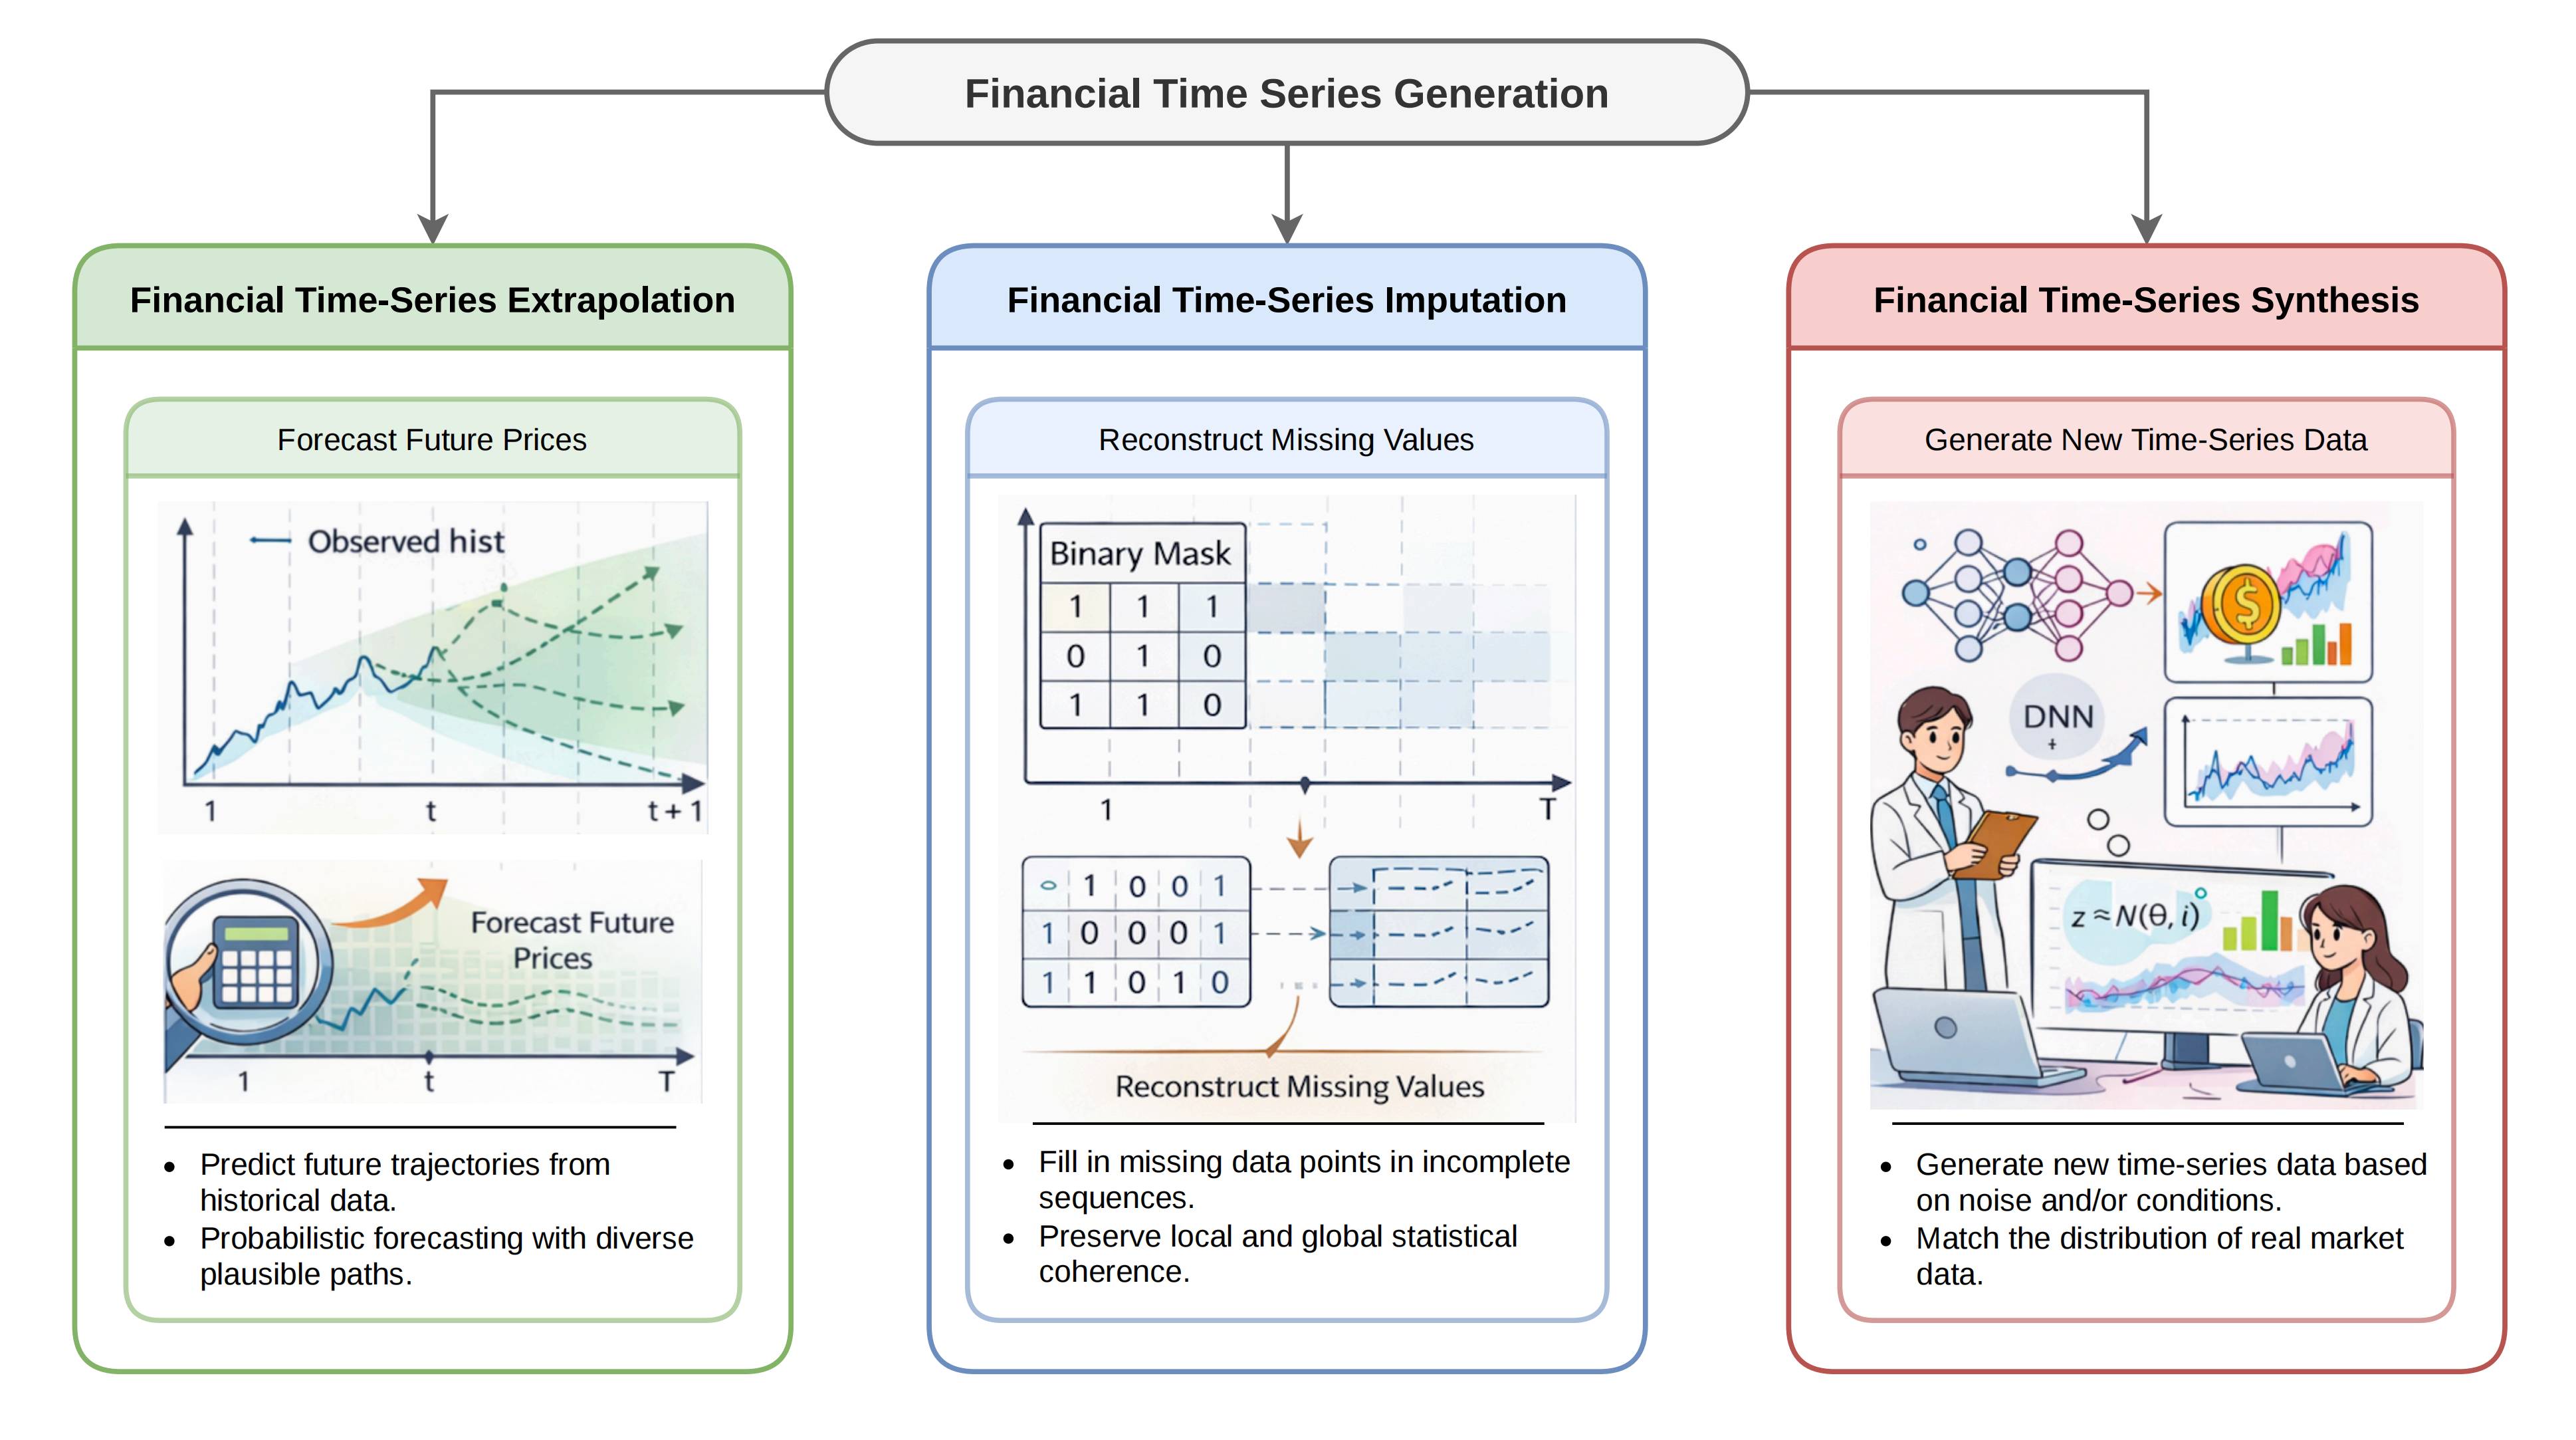
\includegraphics[width=0.9\linewidth]{final_figures/comparison_00.png}
\caption{\textbf{Structural comparison of core financial time-series generation tasks.} Schematic representation contrasting the conditioning context, temporal boundary conditions, and output targets across three generation formulations. \textbf{a,} Financial time-series extrapolation (FTSE): conditional forward-looking trajectory continuation, where a past historical prefix (solid line markers) guides probabilistic generation of unobserved future steps (dashed continuation markers). \textbf{b,} Financial time-series imputation (FTSI): closed-format bidirectional reconstruction, where known observed points bound an interval of missing or corrupted values, reconstructed via temporal and cross-sectional conditioning. \textbf{c,} Synthetic sequence generation (FTSS): unconditional or attribute-guided manifold creation from latent Gaussian noise and market condition vectors, simulating realistic synthetic price paths and order books without pointwise historical alignment.}
\label{fig:tasks}
\end{figure}

\newpage

\begin{figure}[!ht]
\centering
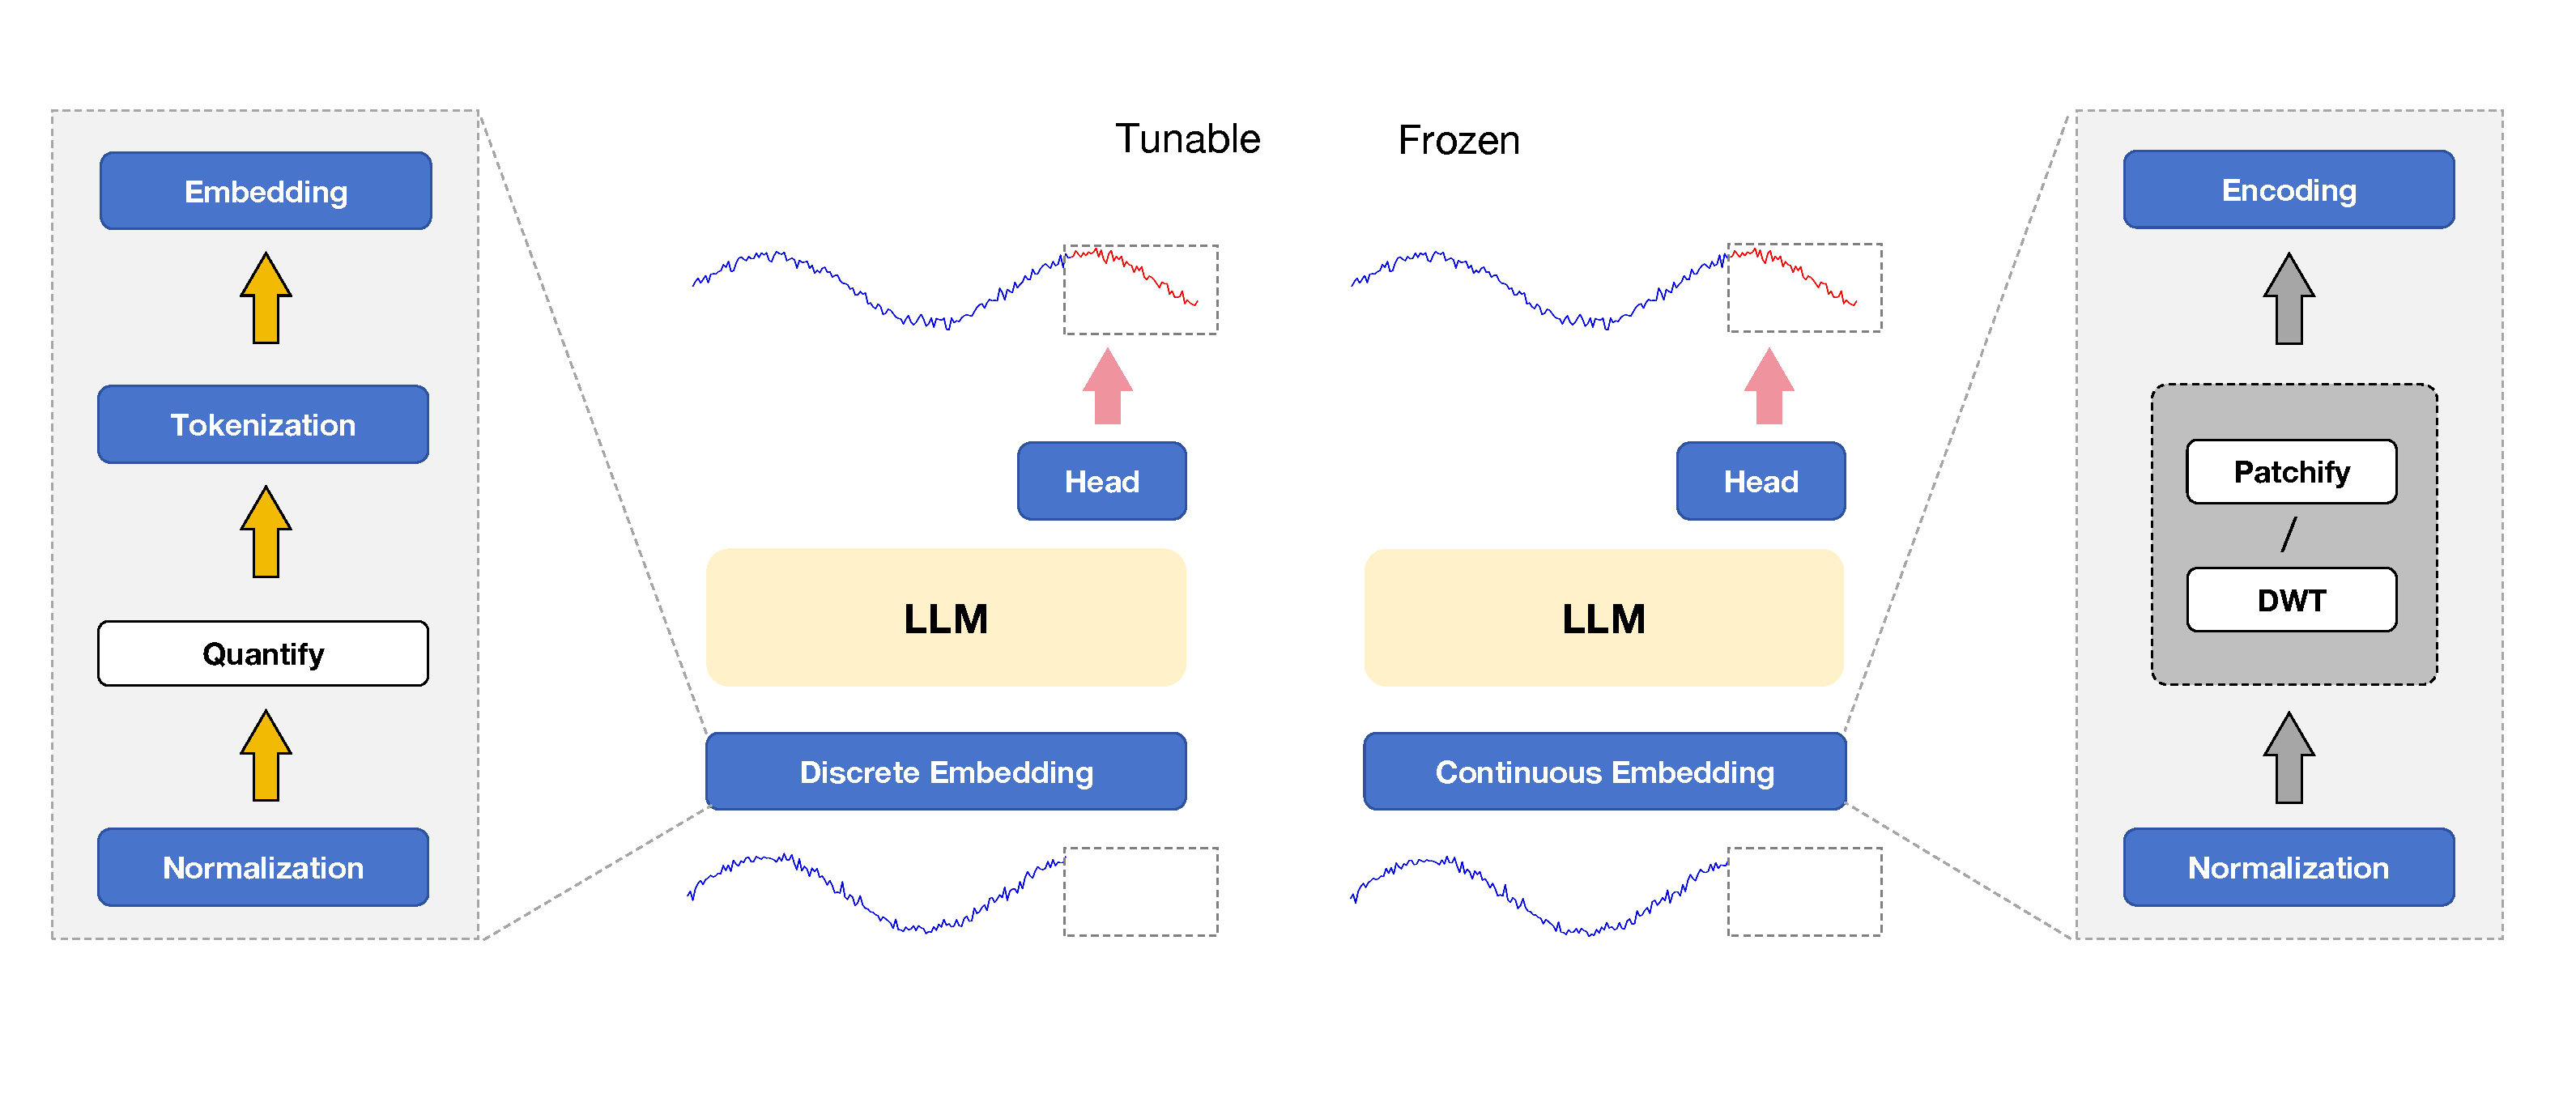
\includegraphics[width=0.8\textwidth,keepaspectratio]{final_figures/DiffWithDiscreteContinous.pdf}
\caption{\textbf{Architectural paradigms for adapting foundation models to financial time series.} Schematic diagram contrasting tokenization- and patch-based fine-tuning against model editing and prompt reprogramming. \textbf{a,} Fine-tuning paradigm (left): numerical continuous time series are transformed into discrete token vocabularies via quantile binning or linear patch projection layers, followed by backpropagation through transformer backbones. \textbf{b,} Prompt reprogramming and cross-modal model editing paradigm (right): a frozen foundation model backbone receives auxiliary steering signals from textual market prompts, cross-attention alignment bridges, and lightweight adapter modules, avoiding full-parameter gradient updates while preserving numerical precision. Blue rectangular boxes represent time-series input vectors, purple layered blocks denote multi-head self-attention transformer layers, and green highlighted modules represent learnable cross-modal projection heads.}
\label{fig:llm_comparison}
\end{figure}

\newpage

\begin{figure}[!ht]
\centering
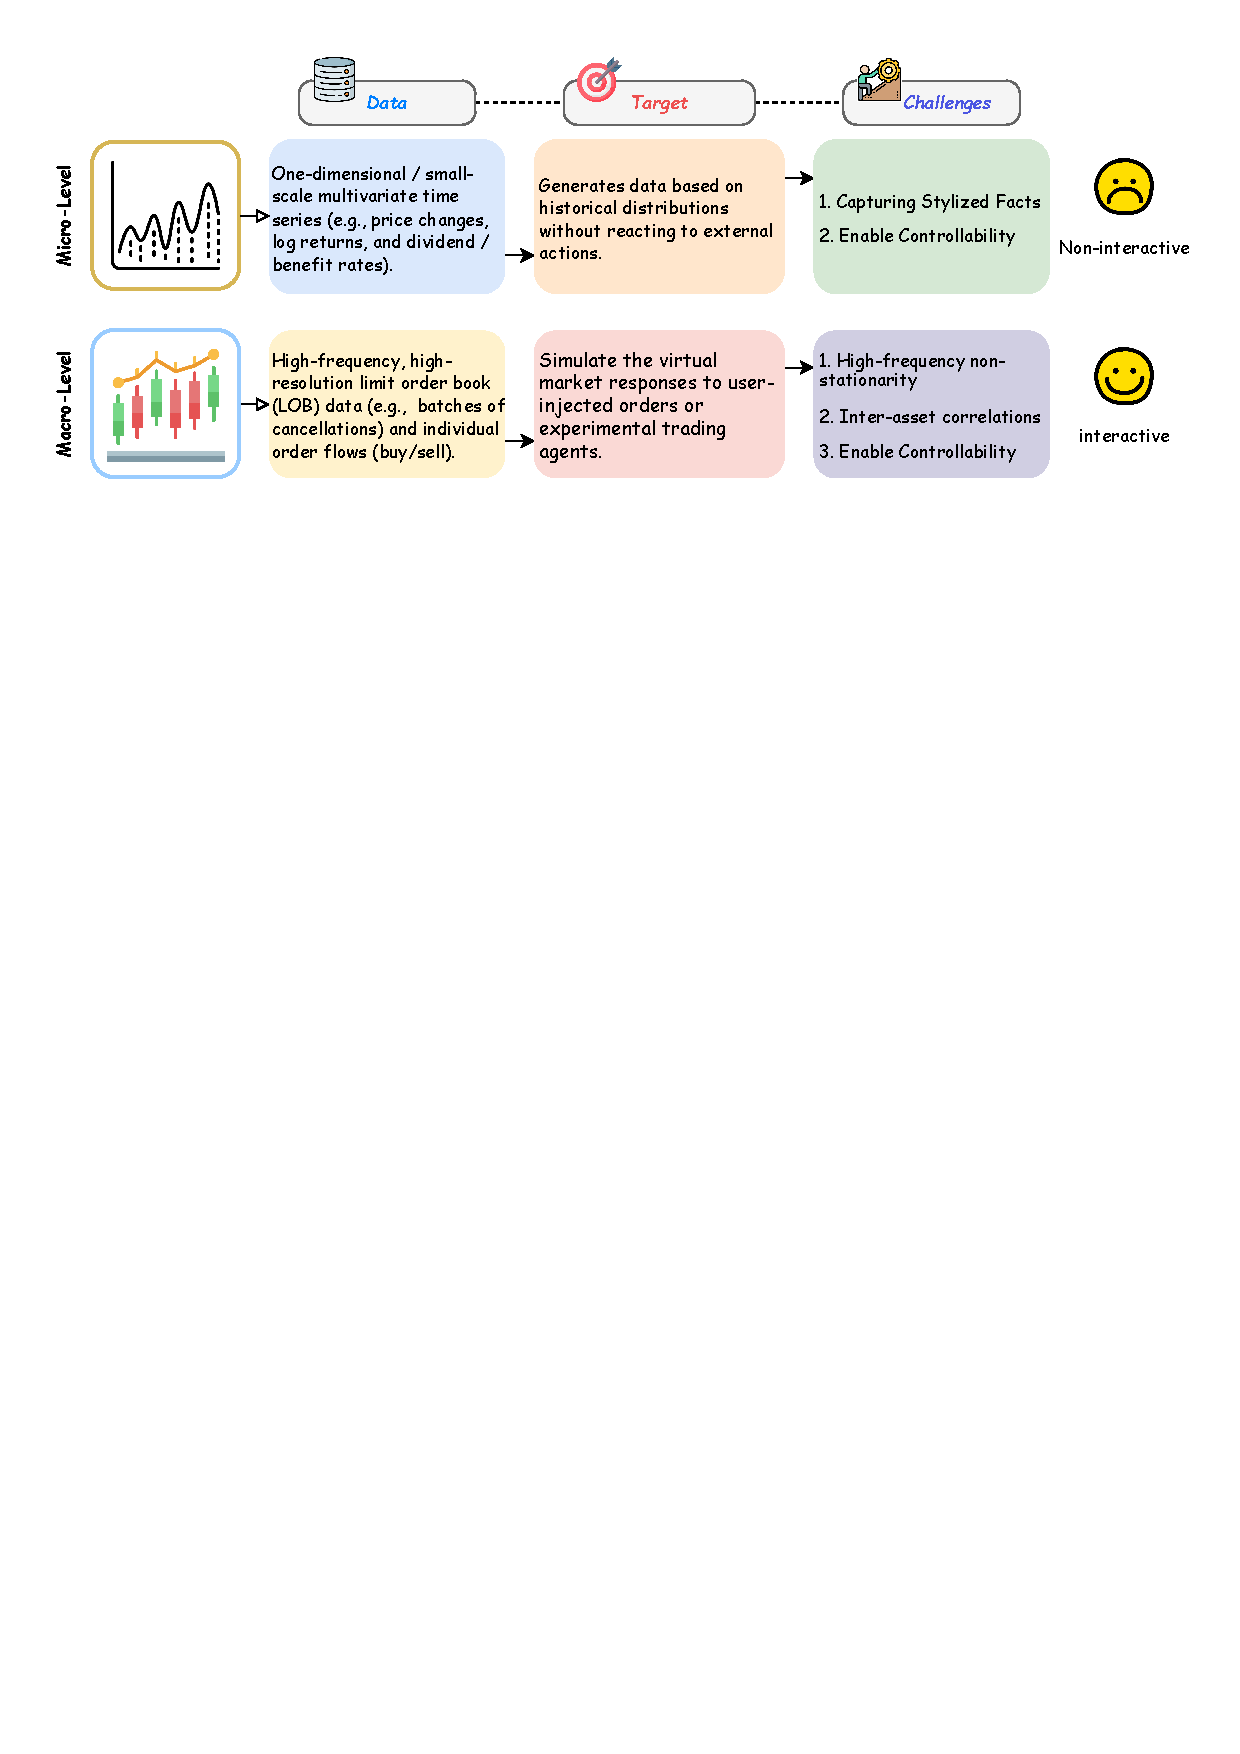
\includegraphics[width=0.8\textwidth,keepaspectratio]{final_figures/FTSA.pdf}
\caption{\textbf{Multi-scale architectural paradigms for financial time-series synthesis.} Conceptual comparison of synthetic sequence generation partitioned into micro-level return modeling and macro-level market simulation. \textbf{a,} Micro-level synthesis (left): univariate or low-dimensional asset return path generation via Wasserstein GANs with temporal convolutional backbones and score-matching diffusion models, engineered to preserve stylized econometric facts such as heavy tails, absence of linear autocorrelation, and volatility clustering. \textbf{b,} Macro-level market simulation (right): multi-agent and limit order book (LOB) queue modeling where generative architectures simulate asynchronous order message flows, bid-ask depth ladders, cross-asset spillover correlations, and macroeconomic counterfactual shock scenarios under regulatory and privacy constraints. Color shading highlights the transition from low-dimensional statistical moments to high-dimensional interactive market topologies.}
\label{fig:ftss_comparison}
\end{figure}

\newpage

\begin{figure}[!ht]
\centering
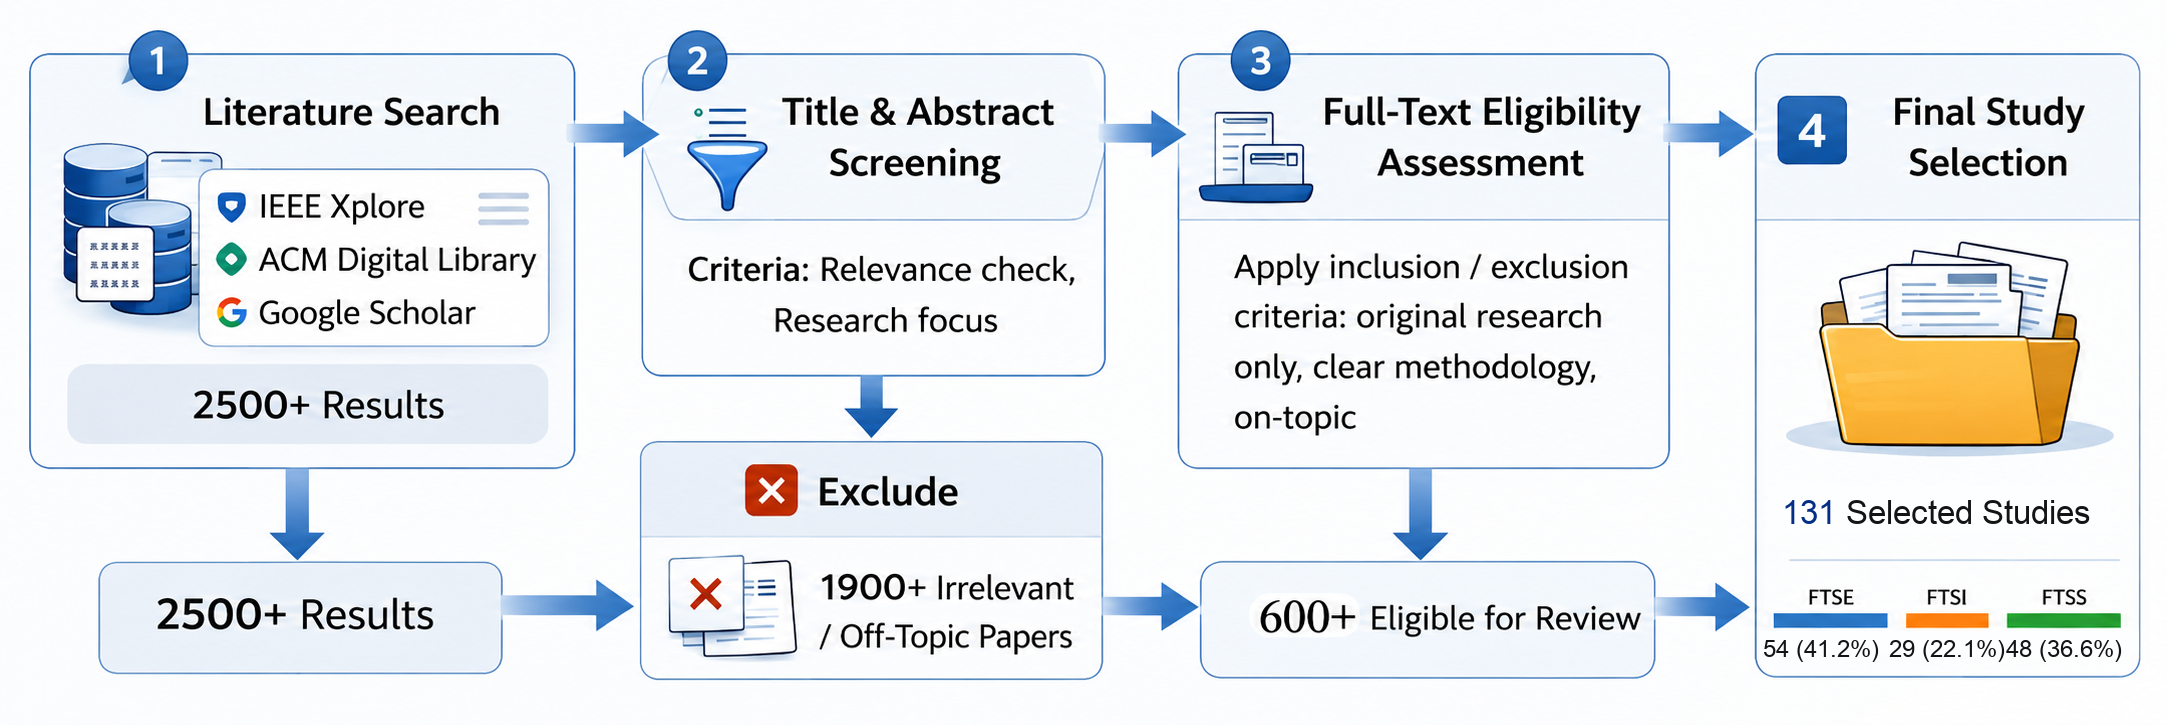
\includegraphics[width=0.95\textwidth,keepaspectratio]{final_figures/filter_pipeline.png}
\caption{\textbf{Literature identification and PRISMA screening pipeline.} Flow diagram illustrating the systematic retrieval, multi-stage screening, and eligibility determination process compliant with the PRISMA 2020 framework. Blue rectangular boxes represent initial literature identification across primary databases (Google Scholar, DBLP, Web of Science, Scopus, arXiv) and duplicate removal. Orange rectangular boxes denote title and abstract screening stages with corresponding exclusion criteria. Red dashed borders and rightward branching callouts indicate excluded records at each phase along with explicit rationales (non-financial domains, deterministic point forecasting without generative distributions, non-reproducible records). Green solid rectangular boxes indicate the final corpus of 130 retained studies meeting all eligibility criteria, partitioned into three task categories: financial time-series extrapolation, imputation, and data synthesis. Detailed quantitative counts for each filtering phase are recorded in the accompanying retrieval statistics table.}
\label{fig:lit_dist}
\end{figure}
